\begin{dang}{Hàm số liên tục trên khoảng, đoạn}
	\begin{itemize}
		\item Hàm số $y=f(x)$ được gọi là liên tục trên một khoảng nếu nó liên tục tại mọi điểm của khoảng đó.\\
		\item Hàm số $y=f(x)$ được gọi là liên tục trên đoạn $[a,b]$ nếu nó liên tục trên khoảng $(a,b)$ và $$\mathop {\lim }\limits_{x \to {a^ + }} f\left( x \right) = f\left( a \right),{\rm{   }}\mathop {\lim }\limits_{x \to {b^ - }} f\left( x \right) = f\left( b \right).$$
		\item Đồ thị của hàm số liên tục trên một khoảng là một đường liền nét trên khoảng đó.
	\end{itemize}
\end{dang}
\subsubsection{Ví dụ mẫu}
\begin{vd}[TH]%[1K5KG-5]% 
	Cho hàm số $f\left( x \right)=\left\{ \begin{aligned}
		& \dfrac{x^2-3x+2}{\sqrt{x+2}-2}\,\,\,\,\,\,\,\,\,khi\,\,x>2 \\
		& {m^2}x-4m+6\,\,\,\,khi\,\,\,x\le 2 \\
	\end{aligned} \right.$, $m$ là tham số. Với giá trị nào của $m$ thì hàm số đã cho liên tục tại $x=2$?
	\dapso{$m=1.$}
	\loigiai{
		Ta có\\
		$\lim\limits_{x\to {2^{+}}} f(x)=\lim\limits_{x\to {2^{+}}} \dfrac{x^2-3x+2}{\sqrt{x+2}-2}=\lim\limits_{x\to {2^{+}}} \dfrac{\left( x-2 \right)\left( x-1 \right)\left( \sqrt{x+2}+2 \right)}{x-2}=\lim\limits_{x\to {2^{+}}} \left( x-1 \right)\left( \sqrt{x+2}+2 \right)=4$.\\
		$\lim\limits_{x\to {2^{-}}} f(x)=\lim\limits_{x\to {2^{-}}} \left( {m^2}x-4m+6 \right)=2m^2-4m+6$.\\
		$f(2)=2m^2-4m+6$.\\
		Để hàm số liên tục tại $x=2$ thì $\lim\limits_{x\to {2^{+}}} f(x)=\lim\limits_{x\to {2^{-}}} f(x)=f(2)\Leftrightarrow 2m^2-4m+6=4\Leftrightarrow 2m^2-4m+2=0\Leftrightarrow m=1$.\\
		Vậy có một giá trị của $m$ thỏa mãn hàm số đã cho liên tục tại $x=2$.}
\end{vd}
\begin{vd}[TH]%[1K5KG-5]% 
	
	Tìm giá trị của tham số $m$ để hàm số $f\left( x \right)=\left\{ \begin{aligned}
		& \dfrac{x^2+3x+2}{x^2-1}\,\,\,\,\,\text{khi}\,\,\,\,\,\,x\,<\,-1 \\
		& mx+2\,\,\,\,\,\,\,\,\,\,\,\,\,\,\,\text{khi}\,\,\,\,\,\,x\,\ge \,-1 \\
	\end{aligned} \right.$ liên tục tại $x=-1$?
	\dapso{$m=\dfrac{5}{2}$.}
	\loigiai{
		Ta có  \\
		$\bullet$ $f\left( -1 \right)=-m+2$.\\
		$\bullet$ $\lim\limits_{x\to {{\left( -1 \right)}^{+}}} f\left( x \right)=-m+2$.\\
		$\bullet$$\lim\limits_{x\to {{\left( -1 \right)}^{-}}} f\left( x \right)=\lim\limits_{x\to {{\left( -1 \right)}^{-}}} \dfrac{x^2+3x+2}{x^2-1}=\lim\limits_{x\to {{\left( -1 \right)}^{-}}} \dfrac{\left( x+1 \right)\left( x+2 \right)}{\left( x-1 \right)\left( x+1 \right)}=\lim\limits_{x\to {{\left( -1 \right)}^{-}}} \dfrac{x+2}{x-1}=\dfrac{-1}{2}$.\\
		Hàm số liên tục tại $x=-1\Leftrightarrow f\left( -1 \right)=\lim\limits_{x\to {{\left( -1 \right)}^{+}}} f\left( x \right)=\lim\limits_{x\to {{\left( -1 \right)}^{-}}} f\left( x \right)\Leftrightarrow -m+2=\dfrac{-1}{2}\Leftrightarrow m=\dfrac{5}{2}$.}
\end{vd}
\begin{vd}[TH]%[1K5BG-5]% 
	Tìm $m$ để hàm số $f\left( x \right)=\left\{ \begin{aligned}
		& \dfrac{x^2-16}{x-4}\,\,\,khi\,x>4 \\
		& mx+1\,\,\,\,\,\,khi\,x\le 4 \\
	\end{aligned} \right.\,$ liên tục tại điểm $x=4$.
	\dapso{ $m=\dfrac{7}{4}$.}
	\loigiai{
		Ta có $\lim\limits_{x\to {4^{-}}} f\left( x \right)=f\left( 4 \right)=4m+1$; $\lim\limits_{x\to {4^{+}}} f\left( x \right)=\lim\limits_{x\to {4^{+}}} \dfrac{x^2-16}{x-4}=\lim\limits_{x\to {4^{+}}} \,\left( x+4 \right)=8$.\\
		Hàm số liên tục tại điểm $x=4\Leftrightarrow \lim\limits_{x\to {4^{-}}} f\left( x \right)=\lim\limits_{x\to {4^{+}}} f\left( x \right)=f\left( 4 \right)\Leftrightarrow 4m+1=8\Leftrightarrow m=\dfrac{7}{4}$.}
\end{vd}
\begin{vd}[TH]%[1K5BG-5]% 
	Tìm $m$ để hàm số $f(x)=\left\{ \begin{aligned}
		& \dfrac{x^2-x-2}{x+1} \text{ khi} x>-1 \\
		& mx-2m^2 \text{ khi }x\le -1 \\
	\end{aligned} \right.$ liên tục tại $x=-1.$
	\dapso{ $m\in \left\{ 1;-\dfrac{3}{2} \right\}$.}
	\loigiai{
		Tập xác định $\mathscr{D}=\mathbb{R}$.\\
		$\bullet$ $f(-1)=-m-2m^2$\\
		$\bullet$ $\lim\limits_{x\to -{1^{-}}} f(x)=\lim\limits_{x\to -{1^{-}}} (mx-2m^2)=-m-2m^2$.\\
		$\bullet$ $\lim\limits_{x\to -{1^{+}}} f(x)=\lim\limits_{x\to -{1^{+}}} \dfrac{x^2-x-2}{x+1}=\lim\limits_{x\to -{1^{+}}} \dfrac{(x+1)(x-2)}{x+1}=\lim\limits_{x\to -{1^{+}}} (x-2)=-3.$\\
		Hàm số liên tục tại $x=-1$ khi và chỉ khi$\lim\limits_{x\to -{1^{-}}} f(x)=\lim\limits_{x\to -{1^{+}}} f(x)=f(-1)$\\
		$\Leftrightarrow -m-2m^2=-3\Leftrightarrow 2m^2+m-3=0\Leftrightarrow \left[ \begin{aligned}
			& m=1 \\
			& m=-\dfrac{3}{2} \\
		\end{aligned} \right..$\\
		Vậy các giá trị của m là $m\in \left\{ 1;-\dfrac{3}{2} \right\}.$}
\end{vd}
\begin{vd}[VD]%[1K5KG-5]% 
	Tìm giá trị của $m$ để hàm số $f\left( x \right)=\left\{ \begin{array}{*{35}{l}}
		\dfrac{\sqrt{1-x}-\sqrt{1+x}}{x} & \text{khi} & x<0 \\
		m+\dfrac{1-x}{1+x} & \text{khi} & x\ge 0 \\
	\end{array} \right.$ liên tục tại $x=0$?
	\dapso{$m=-2$.}
	\loigiai{
		Ta có\\
		$\lim\limits_{x\to {0^{+}}} f\left( x \right)=\lim\limits_{x\to {0^{+}}} \left( m+\dfrac{1-x}{1+x} \right)=m+1$.
		$\lim\limits_{x\to {0^{-}}} f\left( x \right)=\lim\limits_{x\to {0^{-}}} \left( \dfrac{\sqrt{1-x}-\sqrt{1+x}}{x} \right)=\lim\limits_{x\to {0^{-}}} \dfrac{-2x}{x\left( \sqrt{1-x}+\sqrt{1+x} \right)}=\lim\limits_{x\to {0^{-}}} \dfrac{-2}{\left( \sqrt{1-x}+\sqrt{1+x} \right)}=-1$.\\
		$f\left( 0 \right)=m+1$.\\
		Để hàm liên tục tại $x=0$ thì $\lim\limits_{x\to {0^{+}}} f\left( x \right)=\lim\limits_{x\to {0^{-}}} f\left( x \right)=f\left( 0 \right)\Leftrightarrow m+1=-1\Rightarrow m=-2$.}
\end{vd}
\subsubsection{Bài tập rèn luyện}
\centerline{\fcolorbox{red}{yellow!50}{\bf {BÀI TẬP TỰ LUẬN}}}
\begin{bt}[TH]%[1K5KG-5]%
	
	Cho hàm số $f\left( x \right)=\left\{ \begin{aligned}
		& \dfrac{\sqrt{x+3}-2}{x-1}\text{khi }\left( x>1 \right) \\
		& {m^2}+m+\dfrac{1}{4}\text{  }\text{khi }\left( x\le 1 \right) \\
	\end{aligned} \right.$. Tìm tất cả các giá trị của tham số thực $m$ để hàm số $f\left( x \right)$ liên tục tại $x=1$?
	\dapso{$m\in \left\{ 0;-1 \right\}$.}
	\loigiai{
		Ta có $\lim\limits_{x\to {1^{+}}} f\left( x \right)=\lim\limits_{x\to {1^{+}}} \dfrac{\sqrt{x+3}-2}{x-1}=\lim\limits_{x\to {1^{+}}} \dfrac{1}{\sqrt{x+3}+2}=\dfrac{1}{4}$; $f\left( 1 \right)=\lim\limits_{x\to {1^{-}}} f\left( x \right)=m^2+m+\dfrac{1}{4}$.\\
		Để hàm số $f\left( x \right)$ liên tục tại $x=1$ thì $m^2+m+\dfrac{1}{4}=\dfrac{1}{4}\Leftrightarrow \left[ \begin{aligned}
			& m=-1 \\
			& m=0 \\
		\end{aligned} \right.$.}
\end{bt}
\begin{bt}[TH]%[1K5KG-5]%
	
	Tìm $a$ để hàm số  $f\left( x \right)=\left\{ \begin{aligned}
		& 2x+a\,\,\,\,\,\,\,\,\,\,\,\,\,\,\,\,\,\,\,\,\,\,\,\text{khi}\,\,\,x\le 1 \\
		& \dfrac{x^3-x^2+2x-2}{x-1}\,\,\,\text{khi}\,\,\,x>1 \\
	\end{aligned} \right.$ liên tục trên $\mathbb{R}$?
	\dapso{$a=1.$}
	\loigiai{
		Khi $x<1$ thì $f\left( x \right)=2x+a$ là hàm đa thức nên liên tục trên khoảng $\left( -\infty ;\,1 \right)$.\\
		Khi $x>1$ thì $f\left( x \right)=\dfrac{x^3-x^2+2x-2}{x-1}$ là hàm phân thức hữu tỉ xác định trên khoảng $\left( 1;\,+\infty \right)$ nên liên tục trên khoảng $\left( 1;\,+\infty \right)$.\\
		Xét tính liên tục của hàm số tại điểm $x=1$, ta có  \\
		+ $f\left( 1 \right)=2+a$.\\
		+ $\lim\limits_{x\,\to \,{1^{-}}} f\left( x \right)=\lim\limits_{x\,\to \,{1^{-}}} \left( 2x+a \right)=2+a$.\\
		+ $\lim\limits_{x\,\to \,{1^{+}}} f\left( x \right)=\lim\limits_{x\,\to \,{1^{+}}} \dfrac{x^3-x^2+2x-2}{x-1}=\lim\limits_{x\,\to \,{1^{+}}} \dfrac{\left( x-1 \right)\left( {x^2}+2 \right)}{x-1}=\lim\limits_{x\,\to \,{1^{+}}} \left( {x^2}+2 \right)=3$.\\
		Hàm số $f\left( x \right)$ liên tục trên $\mathbb{R}$ $\Leftrightarrow $ hàm số $f\left( x \right)$ liên tục tại $x=1$.\\
		$\lim\limits_{x\,\to \,{1^{-}}} f\left( x \right)=\lim\limits_{x\,\to \,{1^{+}}} f\left( x \right)=f\left( 1 \right)$ $\rightarrow$ $2a+1=3$ $\rightarrow$ $a=1$.}
\end{bt}
\begin{bt}[TH]%[1K5KG-5]% 
	
	Tìm $m$ để hàm số $f(x)=\left\{ \begin{aligned}
		& \dfrac{x^2+4x+3}{x+1}\,\,\,khi\,\,x>-1 \\
		& mx+2\,\,\,\,\,\,\,\,\,\,\,\,\,khi\,\,x\le -1 \\
	\end{aligned} \right.$ liên tục tại điểm $x=-1$.
	\dapso{$m=2$.}
	\loigiai{
		Ta có   $\lim\limits_{x\to {{\left( -1 \right)}^{+}}} f\left( x \right)=\lim\limits_{x\to {{\left( -1 \right)}^{+}}} \dfrac{x^2+4x+3}{x+1}=\lim\limits_{x\to {{\left( -1 \right)}^{+}}} \dfrac{\left( x+1 \right)\left( x+3 \right)}{x+1}=\lim\limits_{x\to {{\left( -1 \right)}^{+}}} \left( x+3 \right)=2$.\\
		$\lim\limits_{x\to {{\left( -1 \right)}^{-}}} f\left( x \right)=\lim\limits_{x\to {{\left( -1 \right)}^{-}}} \left( mx+2 \right)=-m+2$.\\
		$f\left( -1 \right)=-m+2$.\\
		Để hàm số đã cho liên tục tại điểm $x=-1$ thì $\lim\limits_{x\to {{\left( -1 \right)}^{+}}} f\left( x \right)=\lim\limits_{x\to {{\left( -1 \right)}^{-}}} f\left( x \right)=f\left( -1 \right)\Leftrightarrow 2=-m+2\Leftrightarrow m=0$.}
\end{bt}
\begin{bt}[VD]%[1K5BG-4]% 
	
	Cho hàm số $f\left( x \right)=\left\{ \begin{matrix}
		\sin \pi x & \text{khi}\,\,\left| x \right|\le 1 \\
		x+1\ & \text{khi}\,\ \left| x \right|>1 \\
	\end{matrix} \right.$. Tìm các khoảng liên tục của hàm số?
	\dapan{ Hàm số liên tục trên các khoảng $\left( -\infty ;1 \right)$ và $\left( 1;+\infty \right)$.}
	\loigiai{
		Ta có   $\lim\limits_{x\to {1^{+}}} \left( x+1 \right)=2$ và $\lim\limits_{x\to {1^{-}}} \sin \pi x=0\Rightarrow \lim\limits_{x\to {1^{+}}} f\left( x \right)\ne \lim\limits_{x\to {1^{-}}} f\left( x \right)$ do đó hàm số gián đoạn tại $x=1$.\\
		Tương tự $\lim\limits_{x\to {{\left( -1 \right)}^{-}}} \left( x+1 \right)=0$ và $\lim\limits_{x\to {{\left( -1 \right)}^{+}}} \sin \pi x=0$\\
		$\Rightarrow \lim\limits_{x\to {{\left( -1 \right)}^{+}}} f\left( x \right)=\lim\limits_{x\to {{\left( -1 \right)}^{-}}} f\left( x \right)=\lim\limits_{x\to -1} f\left( x \right)=f\left( -1 \right)$ do đó hàm số liên tục tại $x=-1$.\\
		Với $x\ne \pm 1$ thì hàm số liên tục trên tập xác định.\\
		Vậy hàm số đã cho liên tục trên các khoảng $\left( -\infty ;1 \right)$ và $\left( 1;+\infty \right)$.}
\end{bt}
\begin{bt}[TH]%[1K5KG-4]%
	
	Cho hàm số $f\left( x \right)=\left\{ \begin{aligned}
		& \sin x\,\,\,\,\text{nếu}\,\cos x\ge 0 \\
		& 1+\cos x\,\,\,\,\text{nếu}\,\cos x<0 \\
	\end{aligned} \right..$ Hỏi hàm số $f$ có tất cả bao nhiêu điểm gián đoạn trên khoảng $\left( 0;2018 \right)$?
	\dapso{$642$.}
	\loigiai{
		Vì $f$ là hàm lượng giác nên hàm số $f$ gián đoạn khi và chỉ khi hàm số $f$ gián đoạn tại $x$ làm cho $\cos x=0$ $\Leftrightarrow x=\dfrac{\pi }{2}+k\pi \,\left( k\in \mathbb{Z} \right)\in \left( 0;2018 \right)$ $\Leftrightarrow 0<\dfrac{\pi }{2}+k\pi <2018\Leftrightarrow 0<\dfrac{1}{2}+k<\dfrac{2018}{\pi }$ $\Leftrightarrow -\dfrac{1}{2}<k<\dfrac{2018}{\pi }-\dfrac{1}{2}\Leftrightarrow 0\le k\le 641$.}
\end{bt}
\begin{bt}[TH]%[1K5KG-5]%
	
	Tìm $m$ để hàm số $y=f\left( x \right)=\left\{ \begin{aligned}
		& {x^2}+2\sqrt{x-2}\,\,\,\,\,\,\,khi\,x\ge 2 \\
		& 5x-5m+m^2\,\,\,\,\,\,\,khi\,x<2 \\
	\end{aligned} \right.$ liên tục trên $\mathbb{R}$?
	\dapso{$m=2; m=3$.}
	\loigiai{
		Tập xác định  $\mathbb{R}\,.$\\
		+ Xét trên $\left( 2;\,+\infty \right)$ khi đó $f\left( x \right)=x^2+2\sqrt{x-2}$.\\
		$\forall {x_0}\,\in \left( 2;\,+\infty \right), \,\lim\limits_{x\to {x_0}} \left( {x_0}^2\,+2\sqrt{x_0-2} \right)=x_0^2\,+2\sqrt{x_0-2}=f\left( {x_0} \right)\,\Rightarrow $hàm số liên tục trên $\left( 2;\,+\infty \right)$.\\
		+ Xét trên $\left( -\infty ;\,2 \right)$ khi đó $f\left( x \right)=5x-5m+m^2$ là hàm đa thức liên tục trên $\mathbb{R}\,\Rightarrow $ hàm số liên tục trên $\left( -\infty ;\,2 \right)$.\\
		+ Xét tại $x_0=2$, ta có  $f\left( 2 \right)=4$.\\
		$\lim\limits_{x\to {2^{+}}} f\left( x \right)=\lim\limits_{x\to {2^{+}}} \left( {x^2}+2\sqrt{x-2} \right)=4;\,\lim\limits_{x\to {2^{-}}} f\left( x \right)=\lim\limits_{x\to {2^{-}}} \left( 5x-5m+m^2 \right)=m^2-5m+10$.
		Để hàm số đã cho liên tục trên $\mathbb{R}$ thì nó phải liên tục tại $x_0=2$.\\
		$\Leftrightarrow \lim\limits_{x\to {2^{+}}} f\left( x \right)=\,\lim\limits_{x\to {2^{-}}} f\left( x \right)=f\left( 2 \right)\Leftrightarrow {m^2}-5m+10=4\,\Leftrightarrow {m^2}-5m+6=0\,\Leftrightarrow \left[ \begin{aligned}
			& m=2 \\
			& m=3 \\
		\end{aligned} \right.$.}
\end{bt}
\begin{bt}[VD]%[1K5KG-5]%  
	
	Cho hàm số $f\left( x \right)=\left\{ \begin{aligned}
		& \,3x+a-1\,\,\,\,khi\,\,\,x\le 0 \\
		& \dfrac{\sqrt{1+2x}-1}{x}\,\,khi\,\,\,x>0 \\
	\end{aligned} \right.$. Tìm tất cả giá trị thực của a để hàm số đã cho liên tục trên $\mathbb{R}$.
	\dapso{$a=2$.}
	\loigiai{
		Hàm số liên tục tại mọi điểm $x\ne 0$ với mọi a.\\
		Với $x=0$, ta có $f\left( 0 \right)=\,a\,-1.$\\
		$\lim\limits_{x\to {0^{-}}} f\left( x \right)\,=\,\lim\limits_{x\to {0^{-}}} \left( 3x+a-1 \right)\,=\,a-1$.\\
		$\lim\limits_{x\to {0^{+}}} f\left( x \right)\,=\,\lim\limits_{x\to {0^{+}}} \dfrac{\sqrt{1+2x}-1}{x}\,=\,\lim\limits_{x\to {0^{+}}} \dfrac{2x}{x\left( \sqrt{1+2x}+1 \right)}=\lim\limits_{x\to {0^{+}}} \dfrac{2}{\sqrt{1+2x}+1}=1$.\\
		Hàm số liên tục trên $\mathbb{R}$ khi và chỉ khi hàm số liên tục tại $x=0\Leftrightarrow a-1\,=\,1\Leftrightarrow a=2$.}
\end{bt}
\begin{bt}[TH]%[1K5BG-5]%
	
	Có bao nhiêu giá trị thực của tham số $m$ để hàm số $f\left( x \right)=\left\{ \begin{array}{*{35}{l}}
		m^2{x^2} & \text{khi }x\le 2 \\
		\left( 1-m \right)x & \text{khi }x>2 \\
	\end{array} \right.$ liên tục trên $\mathbb{R}$?
	\dapso{$2$.}
	\loigiai{
		Ta có hàm số luôn liên tục với $\forall x\ne 2$.\\
		Tại $x=2$, ta có $\lim\limits_{x\to {2^{+}}} f\left( x \right)=\lim\limits_{x\to {2^{-}}} \left( 1-m \right)x=\left( 1-m \right)2$;\\
		$\lim\limits_{x\to {2^{-}}} f\left( x \right)=\lim\limits_{x\to {2^{-}}} \left( {m^2}{x^2} \right)=4m^2$; $f\left( 2 \right)=4m^2$.\\
		Hàm số liên tục tại $x=2$ khi và chỉ khi\\
		$\lim\limits_{x\to {2^{+}}} f\left( x \right)=\lim\limits_{x\to {2^{+}}} f\left( x \right)=f\left( 2 \right)\Leftrightarrow 4m^2=\left( 1-m \right)2\Leftrightarrow 4m^2+2m-2=0.\left( 1 \right)$\\
		Phương trình luôn có hai nghiệm thực phân biệt. Vậy có hai giá trị của $m$.\\
	}
\end{bt}
\begin{bt}[th]%[1K5BG-5]%
	
	Tìm $P$ để hàm số $y=\left\{ \begin{aligned}
		& \dfrac{x^2-4x+3}{x-1}\,\,\text{khi}\,\,x>1 \\
		& 6Px-3\,\,\,\,\,\,\,\,\,\text{khi}\,\,x\le 1\,\,\, \\
	\end{aligned} \right.$ liên tục trên $\mathbb{R}$.
	\dapso{$P=\dfrac{1}{6}.$}
	\loigiai{
		Hàm số $y=f\left( x \right)$ liên tục trên $\mathbb{R}\Rightarrow $ $y=f\left( x \right)$ liên tục tại $x=1$
		$\Rightarrow $ $\lim\limits_{x\to {1^{+}}} f\left( x \right)=\lim\limits_{x\to {1^{-}}} f\left( x \right)=f\left( 1 \right)$.\\
		$\lim\limits_{x\to {1^{+}}} f\left( x \right)=\lim\limits_{x\to {1^{+}}} \dfrac{x^2-4x+3}{x-1}=\lim\limits_{x\to {1^{+}}} \left( x-3 \right)=-2$.\\
		$\lim\limits_{x\to {1^{-}}} f\left( x \right)=\lim\limits_{x\to {1^{-}}} \left( 6Px-3 \right)=6P-3$.\\
		$f\left( 1 \right)=6P-3$.\\
		Do đó $\lim\limits_{x\to {1^{+}}} f\left( x \right)=\lim\limits_{x\to {1^{-}}} f\left( x \right)=f\left( 1 \right)$ $\Leftrightarrow 6P-3=-2\Leftrightarrow P=\dfrac{1}{6}$.}
\end{bt}
\begin{bt}[TH]%[1K5BG-5]% 
	
	Hàm số ${f(x)=\left\{ \begin{aligned}
			& ax+b+1,\,\,khi\,\,x>0 \\
			& a\cos x+b\sin x\,,\,khi\,\,x\le 0 \\
		\end{aligned} \right.}$ liên tục trên ${\mathbb{R}}$ khi và chỉ khi
	\dapso{ ${a-b=1}$.}
	\loigiai{
		Khi $x<0$ thì $f\left( x \right)=a\cos x+b\sin x$ liên tục với $x<0$.\\
		Khi $x>0$ thì $f\left( x \right)=ax+b+1$ liên tục với mọi $x>0$.\\
		Tại $x=0$ ta có $f\left( 0 \right)=a$.\\
		${\lim\limits_{x\to {0^{+}}} f\left( x \right)}{=\lim\limits_{x\to {0^{+}}} \left( ax+b+1 \right)}{=b+1}$.\\
		${\lim\limits_{x\to {0^{-}}} f\left( x \right)}{=\lim\limits_{x\to {0^{-}}} \left( a\cos x+b\sin x \right)}{=a}$.\\
		Để hàm số liên tục tại ${x=0}$ thì ${\lim\limits_{x\to {0^{+}}} f\left( x \right)}{=\lim\limits_{x\to {0^{-}}} f\left( x \right)}=f\left( 0 \right)\Leftrightarrow a=b+1\Leftrightarrow a-b=1$.}
\end{bt}
\begin{bt}[TH]%[1K5BG-5]% 
	
	Cho hàm số $y=\left\{ \begin{aligned}
		& 3x+1\quad khi\,x\ge -1 \\
		& x+m\quad khi\,x<-1 \\
	\end{aligned} \right.$, $m$ là tham số. Tìm $m$ để hàm số liên tục trên $\mathbb{R}$.
	\daapso{ $m=-1$}
	\loigiai{
		Ta có hàm số liên tục trên các khoảng $\left( -\infty ;\,-1 \right)$ và $\left( -1;\,+\infty \right)$.\\
		Xét tính liên tục của hàm số tại $x=-1$.\\
		Có $y\left( -1 \right)=-2=\lim\limits_{x\to -{1^{+}}} y$ và $\lim\limits_{x\to -{1^{-}}} y=-1+m$.\\
		Để hàm số liên tục trên $\mathbb{R}$ thì $y\left( -1 \right)=\lim\limits_{x\to -{1^{+}}} y=\lim\limits_{x\to -{1^{-}}} y\Leftrightarrow -2=-1+m\Leftrightarrow m=-1$.}
\end{bt}
\centerline{\fcolorbox{red}{yellow!50}{\bf {CÂU HỎI TRẮC NGHIỆM }}}
\Opensolutionfile{ans}[ans/ans-1K5-3-Dang3]

\begin{ex}%[1K5BG-4]% 
	
	Cho hàm số $y=f\left( x \right)$ liên tục trên $(a;b)$. Điều kiện cần và đủ để hàm số liên tục trên $\left[ a;b \right]$ là
	\choice
	{ $\lim\limits_{x\to {a^{+}}} f\left( x \right)=f\left( a \right)$ và $\lim\limits_{x\to {b^{+}}} f\left( x \right)=f\left( b \right)$}
	{ $\lim\limits_{x\to {a^{-}}} f\left( x \right)=f\left( a \right)$ và $\lim\limits_{x\to {b^{-}}} f\left( x \right)=f\left( b \right)$}
	{\True $\lim\limits_{x\to {a^{+}}} f\left( x \right)=f\left( a \right)$ và $\lim\limits_{x\to {b^{-}}} f\left( x \right)=f\left( b \right)$}
	{ $\lim\limits_{x\to {a^{-}}} f\left( x \right)=f\left( a \right)$ và $\lim\limits_{x\to {b^{+}}} f\left( x \right)=f\left( b \right)$}
	\loigiai{
		Theo định nghĩa hàm số liên tục trên đoạn $\left[ a;b \right]$. Chọn  $\lim\limits_{x\to {a^{+}}} f\left( x \right)=f\left( a \right)$ và $\lim\limits_{x\to {b^{-}}} f\left( x \right)=f\left( b \right)$.}
\end{ex}
\begin{ex}%[1K5KG-1]% 
	
	Cho đồ thị của hàm số $y=f\left( x \right)$ như hình vẽ sau$\colon$ 
	\begin{center}
		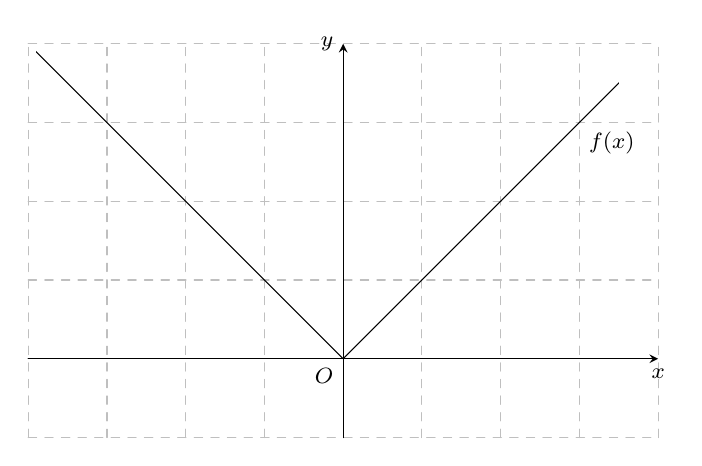
\begin{tikzpicture}[scale=1,>=stealth, font=\footnotesize, line join=round, line cap=round]
			\def\a{1} \def\b{-4} \def\c{3} % Hệ số
			\def\xmin{-4} \def\xmax{4}
			\def\ymin{-1} \def\ymax{4}	
			\draw[color=gray!50,dashed] (\xmin,\ymin) grid (\xmax,\ymax);
			\coordinate [label=below right: $f(x)$] (E) at (3,3);
			\draw[->] (\xmin,0)--(\xmax,0) node [below]{$x$};
			\draw[->] (0,\ymin)--(0,\ymax) node [left]{$y$};
			\node at (0,0) [below left]{$O$};
			\clip (\xmin+0.1,0) rectangle (\xmax-0.5,\ymax-0.1);
			\draw[smooth,samples=300] plot(\x,{1*(\x)});
			\draw[smooth,samples=300] plot(\x,{-1*(\x)});	
		\end{tikzpicture}
	\end{center}
	Chọn mệnh đề đúng.
	\choice
	{ Hàm số $y=f\left( x \right)$ có đạo hàm tại điểm $x=0$ nhưng không liên tục tại điểm $x=0$}
	{\True Hàm số $y=f\left( x \right)$liên tục tại điểm $x=0$ nhưng không có đạo hàm tại điểm $x=0$}
	{ Hàm số $y=f\left( x \right)$ liên tục và có đạo hàm tại điểm $x=0$}
	{ Hàm số $y=f\left( x \right)$ không liên tục và không có đạo hàm tại điểm $x=0$}
	\loigiai{
		Đồ thị là một đường liền nét, nhưng bị “gãy” tại điểm $x=0$ nên nó liên tục tại điểm $x=0$ nhưng không có đạo hàm tại điểm $x=0$.}
\end{ex}
\begin{ex}%[1K5KG-1]% 
	
	Hình nào trong các hình dưới đây là đồ thị của hàm số không liên tục tại $x=1$?
	\choice
	{ 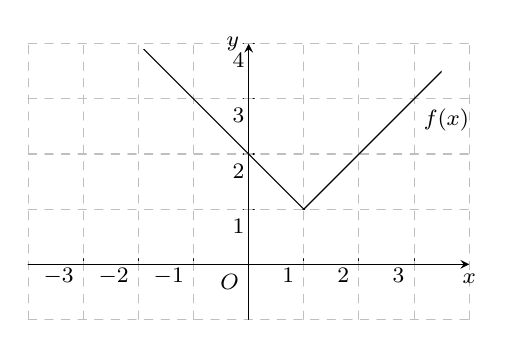
\begin{tikzpicture}[scale=0.7,>=stealth, font=\footnotesize, line join=round, line cap=round]
			\def\a{1} \def\b{-4} \def\c{3} % Hệ số
			\def\xmin{-4} \def\xmax{4}
			\def\ymin{-1} \def\ymax{4}	
			\foreach \x in {-3,-2,-1, 1,2,3}{
				\draw (\x,-.1)--(\x,.1) node[below left]{$\x$};%Oy
			}
			\foreach \y in {1,2,3,4}{
				\draw[-] (-.1,\y)--(.1,\y) node[below left]{$\y$};%Oy
			}
			\draw[color=gray!50,dashed] (\xmin,\ymin) grid (\xmax,\ymax);
			\coordinate [label=below right: $f(x)$] (E) at (3,3);
			\draw[->] (\xmin,0)--(\xmax,0) node [below]{$x$};
			\draw[->] (0,\ymin)--(0,\ymax) node [left]{$y$};
			\node at (0,0) [below left]{$O$};
			\clip (\xmin+0.1,1) rectangle (\xmax-0.5,\ymax-0.1);
			\draw[smooth,samples=300] plot(\x,{1*(\x)});
			\draw[smooth,samples=300] plot(\x,{-1*(\x)+2});	
	\end{tikzpicture}}
	{ 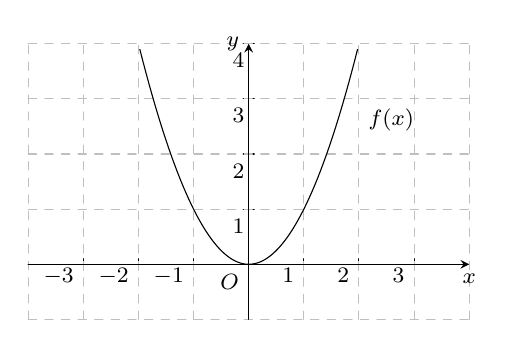
\begin{tikzpicture}[scale=0.7,>=stealth, font=\footnotesize, line join=round, line cap=round]
			\def\a{1} \def\b{-4} \def\c{3} % Hệ số
			\def\xmin{-4} \def\xmax{4}
			\def\ymin{-1} \def\ymax{4}	
			\foreach \x in {-3,-2,-1, 1,2,3}{
				\draw (\x,-.1)--(\x,.1) node[below left]{$\x$};%Oy
			}
			\foreach \y in {1,2,3,4}{
				\draw[-] (-.1,\y)--(.1,\y) node[below left]{$\y$};%Oy
			}
			\draw[color=gray!50,dashed] (\xmin,\ymin) grid (\xmax,\ymax);
			\coordinate [label=below right: $f(x)$] (E) at (2,3);
			\draw[->] (\xmin,0)--(\xmax,0) node [below]{$x$};
			\draw[->] (0,\ymin)--(0,\ymax) node [left]{$y$};
			\node at (0,0) [below left]{$O$};
			\clip (\xmin+0.1,0) rectangle (\xmax-0.5,\ymax-0.1);
			\draw[smooth,samples=300] plot(\x,{1*(\x)^2});	
	\end{tikzpicture}}
	{ 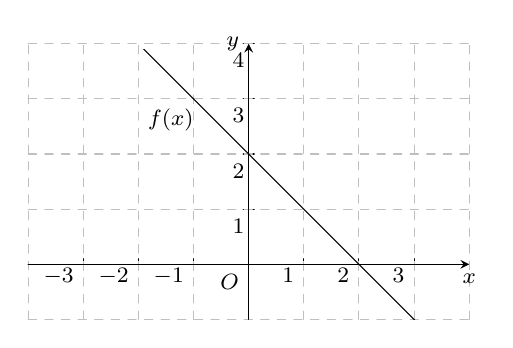
\begin{tikzpicture}[scale=0.7,>=stealth, font=\footnotesize, line join=round, line cap=round]
			\def\a{1} \def\b{-4} \def\c{3} % Hệ số
			\def\xmin{-4} \def\xmax{4}
			\def\ymin{-1} \def\ymax{4}	
			\foreach \x in {-3,-2,-1, 1,2,3}{
				\draw (\x,-.1)--(\x,.1) node[below left]{$\x$};%Oy
			}
			\foreach \y in {1,2,3,4}{
				\draw[-] (-.1,\y)--(.1,\y) node[below left]{$\y$};%Oy
			}
			\draw[color=gray!50,dashed] (\xmin,\ymin) grid (\xmax,\ymax);
			\coordinate [label=below right: $f(x)$] (E) at (-2,3);
			\draw[->] (\xmin,0)--(\xmax,0) node [below]{$x$};
			\draw[->] (0,\ymin)--(0,\ymax) node [left]{$y$};
			\node at (0,0) [below left]{$O$};
			\clip (\xmin+0.1,-1) rectangle (\xmax-0.5,\ymax-0.1);
			\draw[smooth,samples=300] plot(\x,{-1*(\x)+2});
	\end{tikzpicture}}
	{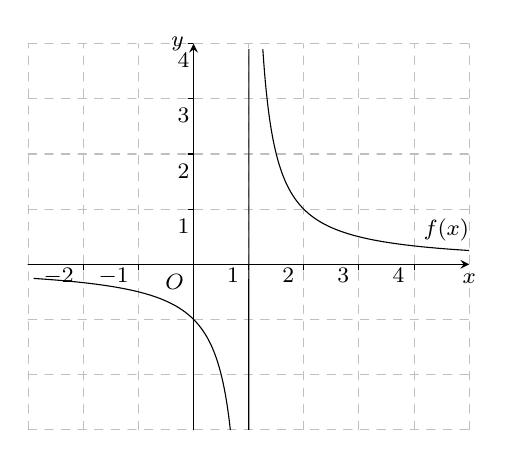
\begin{tikzpicture}[scale=0.7,>=stealth, font=\footnotesize, line join=round, line cap=round]
			\def\a{1} \def\b{-4} \def\c{3} % Hệ số
			\def\xmin{-3} \def\xmax{5}
			\def\ymin{-3} \def\ymax{4}	
			\foreach \x in {-2,-1, 1,2,3,4}{
				\draw (\x,-.1)--(\x,.1) node[below left]{$\x$};%Oy
			}
			\foreach \y in {1,2,3,4}{
				\draw[-] (-.1,\y)--(.1,\y) node[below left]{$\y$};%Oy
			}
			\draw[color=gray!50,dashed] (\xmin,\ymin) grid (\xmax,\ymax);
			\coordinate [label=below right: $f(x)$] (E) at (4,1);
			\draw[->] (\xmin,0)--(\xmax,0) node [below]{$x$};
			\draw[->] (0,\ymin)--(0,\ymax) node [left]{$y$};
			\node at (0,0) [below left]{$O$};
			\clip (\xmin+0.1,-3) rectangle (5,\ymax-0.1);
			\draw [smooth,samples=300] plot (\x, {1/(\x-1)});
	\end{tikzpicture}}
	\loigiai{
		Vì $\lim\limits_{x\to {1^{+}}} y\ne \lim\limits_{x\to {1^{-}}} y$ nên hàm số không liên tục tại $x=1$.}
\end{ex}
\begin{ex}%[1K5BG-3]% 
	
	Cho hàm số $y=\left\{ \begin{aligned}
		& \dfrac{1-x^3}{1-x},\text{khi  }x<1 \\
		& 1\text{  },\text{khi  }x\ge 1 \\
	\end{aligned} \right.$. Hãy chọn kết luận đúng
	\choice
	{\True $y$ liên tục phải tại $x=1$}
	{ $y$ liên tục tại $x=1$}
	{ $y$ liên tục trái tại $x=1$}
	{ $y$ liên tục trên $\mathbb{R}$}
	\loigiai{
		Ta có   $y\left( 1 \right)=1$.\\
		Ta có   $\lim\limits_{x\to {1^{+}}} y=1$; $\lim\limits_{x\to {1^{-}}} y=\lim\limits_{x\to {1^{-}}} \dfrac{1-x^3}{1-x}=\lim\limits_{x\to {1^{-}}} \dfrac{\left( 1-x \right)\left( 1+x+x^2 \right)}{1-x}=\lim\limits_{x\to {1^{-}}} \left( 1+x+x^2 \right)=4$.\\
		Nhận thấy $\lim\limits_{x\to {1^{+}}} y=y\left( 1 \right)$, suy ra $y$ liên tục phải tại $x=1$.}
\end{ex}
\begin{ex}%[1K5BG-4]% 
	
	Trong các hàm số sau, hàm số nào liên tục trên $\mathbb{R}$?
	\choice
	{\True $y=x^3-x$}
	{ $y=\cot x$}
	{ $y=\dfrac{2x-1}{x-1}$}
	{ $y=\sqrt{x^2-1}$}
	\loigiai{
		Vì $y=x^3-x$ là đa thức nên liên tục trên $\mathbb{R}$.}
\end{ex}
\begin{ex}% 
	
	Trong các hàm số sau, hàm số nào liên tục trên $\mathbb{R}$?
	\choice
	{ $f\left( x \right)=\tan x+5$}
	{ $f\left( x \right)=\dfrac{x^2+3}{5-x}$}
	{ $f\left( x \right)=\sqrt{x-6}$}
	{\True $f\left( x \right)=\dfrac{x+5}{x^2+4}$}
	\loigiai{
		Hàm số $f\left( x \right)=\dfrac{x+5}{x^2+4}$ là hàm phân thức hữu tỉ và có tập xác định là $\mathscr{D}=\mathbb{R}$ do đó hàm số $f\left( x \right)=\dfrac{x+5}{x^2+4}$ liên tục trên $\mathbb{R}$.}
\end{ex}
\begin{ex}%[1K5BG-4]%
	
	Cho hàm số $y=\left\{ \begin{aligned}
		& -x^2+x+3\text{  khi}\,\,x\ge 2 \\
		& 5x+2\text{      khi}\,\,x<2 \\
	\end{aligned} \right.$. Chọn mệnh đề sai trong các mệnh đề sau$\colon$ 
	\choice
	{ Hàm số liên tục tại $x_0=1$}
	{\True Hàm số liên tục trên $\mathbb{R}$}
	{ Hàm số liên tục trên các khoảng $\left( -\infty ;\,2 \right),\,\,\left( 2;\,+\infty \right)$}
	{ Hàm số gián đoạn tại $x_0=2$}
	\loigiai{
		+ Với $x>2$, ta có $f\left( x \right)=-x^2+x+3$ là hàm đa thức $\Rightarrow $ hàm số $f\left( x \right)$ liên tục trên khoảng $\left( 2;\,+\infty \right)$.\\
		+ Với $x<2$, ta có $f\left( x \right)=5x+2$ là hàm đa thức $\Rightarrow $ hàm số $f\left( x \right)$ liên tục trên khoảng $\left( -\infty ;\,2 \right)$.\\
		+ Tại $x=2$.\\
		$\lim\limits_{x\to {2^{+}}} f\left( x \right)=\lim\limits_{x\to {2^{+}}} \left( -x^2+x+3 \right)=1$
		$\lim\limits_{x\to {2^{^{-}}}} f\left( x \right)=\lim\limits_{x\to {2^{-}}} \left( 5x+2 \right)=12$
		$\Rightarrow \lim\limits_{x\to {2^{+}}} f\left( x \right)\ne \lim\limits_{x\to {2^{-}}} f\left( x \right)$. Do đó không tồn tại $\lim\limits_{x\to 2} f\left( x \right).$ Vậy hàm số gián đoạn tại $x_0=2$ hay
		Hàm số không liên tục trên $\mathbb{R}$.}
\end{ex}
\begin{ex}%[1K5BG-4]%
	
	Hàm số nào sau đây liên tục trên $\mathbb{R}$?
	\choice
	{ $f\left( x \right)=\sqrt{x}$}
	{\True $f\left( x \right)=x^4-4x^2$}
	{ $f\left( x \right)=\sqrt{\dfrac{x^4-4x^2}{x+1}}$}
	{ $f\left( x \right)=\dfrac{x^4-4x^2}{x+1}$}
	\loigiai{
		Vì hàm số $f\left( x \right)=x^4-4x^2$ có dạng đa thức với   $\mathscr{D}=\mathbb{R}$ nên hàm số này liên tục trên $\mathbb{R}$}
\end{ex}
\begin{ex}%[1K5KG-5]% 
	
	Tìm tất cả các giá trị thực của $m$ để hàm số $f(x)=\left\{ \begin{aligned}
		& \dfrac{\sqrt{x+1}-1}{x}\,\,\,\,\,\,khi\, x>0 \\
		& \sqrt{x^2+1}-m\,\,\,khi\,\,\,x\,\le 0 \\
	\end{aligned} \right.$ liên tục trên $\mathbb{R}$.
	\choice
	{ $m=\dfrac{3}{2}$}
	{\True $m=\dfrac{1}{2}$}
	{ $m=-2$}
	{ $m=-\dfrac{1}{2}$}
	\loigiai{
		Khi $x>0$, ta có   $f(x)=\dfrac{\sqrt{x+1}-1}{x}$ liên tục trên khoảng $\left( 0;+\infty \right)$.\\
		Khi $x<0$, ta có   $f(x)=\sqrt{x^2+1}-m$ liên tục trên khoảng $\left( -\infty ;0 \right)$.\\
		Hàm số liên tục trên $\mathbb{R}$ khi và chỉ khi hàm số liên tục tại $x=0$.\\
		Ta có   $\lim\limits_{x\to {0^{+}}} f(x)=\lim\limits_{x\to {0^{+}}} \dfrac{\sqrt{x+1}-1}{x}=\lim\limits_{x\to {0^{+}}} \dfrac{1}{\sqrt{x+1}+1}=\dfrac{1}{2}$.\\
		$\lim\limits_{x\to {0^{-}}} f(x)=\lim\limits_{x\to {0^{-}}} \left( \sqrt{x^2+1}-m \right)=1-m=f\left( 0 \right)$.
		Do đó hàm số liên tục tại $x=0$ khi và chỉ khi $\dfrac{1}{2}=1-m\Leftrightarrow m=\dfrac{1}{2}$.}
\end{ex}
\begin{ex}%[1K5BG-5]% 
	
	Tìm tất cả các giá trị thực của tham số $m$ để hàm số $f\left( x \right)=\left\{ \begin{array}{*{35}{l}}
		\dfrac{x^2-16}{x-4} & \text{khi} & x>4 \\
		mx+1 & \text{khi} & x\le 4 \\
	\end{array} \right.$ liên tục trên $\mathbb{R}$.
	\choice
	{ $m=8$ hoặc $m=-\dfrac{7}{4}$}
	{\True $m=\dfrac{7}{4}$}
	{ $m=-\dfrac{7}{4}$}
	{ $m=-8$ hoặc $m=\dfrac{7}{4}$}
	\loigiai{
		*) Với $x>4$ thì $f\left( x \right)=\dfrac{x^2-16}{x-4}$ là hàm phân thức nên liên tục trên tập xác định của nó $\Rightarrow f\left( x \right)$ liên tục trên $\left( 4;+\infty \right)$.\\
		*) Với $x<4$ thì $f\left( x \right)=mx+1$ là hàm đa thức nên liên tục trên $\mathbb{R}\Rightarrow f\left( x \right)$ liên tục trên $\left( -\infty ;4 \right)$.\\
		Do vậy hàm số $f\left( x \right)$ đã liên tục trên các khoảng $\left( 4;+\infty \right)$, $\left( -\infty ;4 \right)$.\\
		Suy ra hàm số $f\left( x \right)$ liên tục trên $\mathbb{R}$ khi và chỉ khi $f\left( x \right)$ liên tục tại $x=4$.Do đó\\
		$ \lim\limits_{x\to {4^{+}}} f\left( x \right)=\lim\limits_{x\to {4^{-}}} f\left( x \right)=f\left( 4 \right)\Leftrightarrow \lim\limits_{x\to {4^{+}}} \dfrac{x^2-16}{x-4}=\lim\limits_{x\to {4^{-}}} \left( mx+1 \right)=4m+1\Leftrightarrow \lim\limits_{x\to {4^{+}}} \left( x+4 \right)=4m+1$
		$\Leftrightarrow 4m+1=8\Leftrightarrow m=\dfrac{7}{4}$.}
\end{ex}
\begin{ex}%[1K5KG-5]%
	
	Nếu hàm số $f\left( x \right)=\left\{ \begin{aligned}
		& {x^2}+ax+b\,\,\text{khi}\,\,x<-5\,\, \\
		& x+17\,\,\,\,\,\,\,\,\,\,\,\,\text{khi}\,-5\le x\le 10 \\
		& ax+b+10\,\,\,\text{khi}\,x>10 \\
	\end{aligned} \right.$ liên tục trên $\mathbb{R}$ thì $a+b$ bằng
	\choice
	{\True $-1$}
	{ $0$}
	{ $1$}
	{ $2$}
	\loigiai{
		Với $x<-5$ ta có $f\left( x \right)=x^2+ax+b$, là hàm đa thức nên liên tục trên $\left( -\infty ;-5 \right)$.\\
		Với $-5<x<10$ ta có $f\left( x \right)=x+7$, là hàm đa thức nên liên tục trên $\left( -5;10 \right)$.\\
		Với $x>10$ ta có $f\left( x \right)=ax+b+10$, là hàm đa thức nên liên tục trên $\left( 10;+\infty \right)$.\\
		Để hàm số liên tục trên $\mathbb{R}$ thì hàm số phải liên tục tại $x=-5$ và $x=10$.\\
		Ta có  \\
		$f\left( -5 \right)=12$;$f\left( 10 \right)=17$.\\
		$\lim\limits_{x\to -{5^{-}}} f\left( x \right)=\lim\limits_{x\to -{5^{-}}} \left( {x^2}+ax+b \right)$ $=-5a+b+25$.\\
		$\lim\limits_{x\to -{5^{+}}} f\left( x \right)=\lim\limits_{x\to -{5^{+}}} \left( x+17 \right)=12$.
		$\lim\limits_{x\to {{10}^{-}}} f\left( x \right)=\lim\limits_{x\to {{10}^{-}}} \left( x+17 \right)=27$.
		$\lim\limits_{x\to {{10}^{+}}} f\left( x \right)=\lim\limits_{x\to {{10}^{+}}} \left( ax+b+10 \right)=10a+b+10$.
		Hàm số liên tục tại $x=-5$ và $x=10$ khi\\
		$\left\{ \begin{aligned}
			& 5a+b+25=12 \\
			& 10a+b+10=27 \\
		\end{aligned} \right.\Leftrightarrow \left\{ \begin{aligned}
			& -5a+b=-13 \\
			& 10a+b=17 \\
		\end{aligned} \right.\Leftrightarrow \left\{ \begin{aligned}
			& a=2 \\
			& b=-3 \\
		\end{aligned} \right.\Rightarrow a+b=-1$.}
\end{ex}
\Closesolutionfile{ans}